\documentclass[11pt,a4paper]{article}
\usepackage[a4paper,left=27mm,right=27mm,top=24mm,bottom=24mm]{geometry}
% Shared look of the Rakshasutra white paper and book.
\usepackage[T1]{fontenc}
\usepackage[utf8]{inputenc}
\usepackage{charter}
\usepackage[scaled=0.9]{helvet}
\usepackage{courier}
\usepackage{amsmath,amssymb}
\usepackage{graphicx}
\usepackage{booktabs,array,longtable}
\usepackage[table]{xcolor}
\usepackage{textcomp}
\usepackage{enumitem}
\usepackage{microtype}
\usepackage{tikz}
\usetikzlibrary{arrows.meta,positioning}
\usepackage[most]{tcolorbox}
\definecolor{rsink}{HTML}{171A2B}
\definecolor{rsred}{HTML}{C0271D}
\definecolor{rspaper}{HTML}{F6F1E7}
\definecolor{rsmuted}{HTML}{6A6F85}
\definecolor{rsindigo}{HTML}{2F4B9A}
\definecolor{rsrule}{HTML}{D9D2C2}
\usepackage[colorlinks=true,allcolors=rsindigo]{hyperref}
\usepackage{xurl}
\urlstyle{same}
% Written by generated/make_numbers.py from results/summary.json. Do not edit.
\newcommand{\ToaSos}{66.82}
\newcommand{\ToaBloom}{138.50}
\newcommand{\ToaChunk}{338.18}
\newcommand{\ToaSosNine}{226.3}
\newcommand{\LossSingle}{57.6}
\newcommand{\LossBatch}{25.3}
\newcommand{\LossRak}{30.5}
\newcommand{\LossRakNd}{21.3}
\newcommand{\LoadSingle}{42.9}
\newcommand{\LoadBatch}{14.6}
\newcommand{\LoadRak}{18.2}
\newcommand{\LoadRakNd}{12.0}
\newcommand{\LossRakLow}{14.3}
\newcommand{\LossRakNdLow}{9.7}
\newcommand{\LossBatchLow}{8.6}
\newcommand{\OversizeBatch}{22}
\newcommand{\LossChunk}{34}
\newcommand{\AirRed}{57.6}
\newcommand{\AirRedNd}{72.1}
\newcommand{\AirVsBatch}{25}
\newcommand{\AirVsBatchNd}{18}
\newcommand{\BloomPays}{960}
\newcommand{\DepTags}{637}
\newcommand{\DepPoles}{32}
\newcommand{\DepLoss}{11.0}
\newcommand{\DepLossNd}{7.3}
\newcommand{\McFrames}{695{,}304}
\newcommand{\McErr}{1.7}
\newcommand{\RangeAbove}{4.1}
\newcommand{\RangeOneM}{82}
\newcommand{\RangeCoded}{174}
\newcommand{\MarginFifty}{20.3}
\newcommand{\Mapl}{145.4}
\newcommand{\MaplUnder}{124.9}
\newcommand{\MarginEightOver}{16.1}
\newcommand{\MarginEightUnder}{4.4}
\newcommand{\MarginFourUnder}{1.7}
\newcommand{\MarginFourOver}{22.2}
\newcommand{\GateTrackM}{22}
\newcommand{\GateHubM}{7.5}
\newcommand{\Iactive}{29.74}
\newcommand{\LifeWarm}{48.2}
\newcommand{\LifeCold}{33.8}
\newcommand{\AdvCoded}{5.95}
\newcommand{\AdvOneM}{0.79}
\newcommand{\IactiveCoded}{113.2}
\newcommand{\LifeWarmCoded}{12.8}
\newcommand{\LifeColdCoded}{9.0}
\newcommand{\DroopUnbuf}{1.61}
\newcommand{\DroopCap}{1.61}
\newcommand{\CapNeed}{895}
\newcommand{\PulseMax}{29.8}
\newcommand{\TauMs}{4.2}
\newcommand{\TetherHit}{0.48}
\newcommand{\TetherAlarm}{98}
\newcommand{\TetherAlarmSim}{98}
\newcommand{\TetherWindow}{811}
\newcommand{\TetherUa}{746}
\newcommand{\ParentLife}{1.9}
\newcommand{\TetherRange}{174}
\newcommand{\TetherGate}{78}
\newcommand{\EvCap}{99.7}
\newcommand{\EvCapDense}{95.0}
\newcommand{\SlowTwo}{25}
\newcommand{\SlowFiveOne}{90}
\newcommand{\ClassAWalk}{216}
\newcommand{\SosMedian}{0.5}
\newcommand{\SosFour}{92}
\newcommand{\SosFirstLoss}{23}
\newcommand{\SosPninefive}{7.0}
\newcommand{\SosFiberP}{0.6}
\newcommand{\SosFourLow}{96}
\newcommand{\BloomFifty}{1.6}
\newcommand{\BloomHundred}{8.7}
\newcommand{\BloomThree}{57}
\newcommand{\BloomCapFive}{78}
\newcommand{\BloomCapOne}{41}
\newcommand{\Clash}{10}
\newcommand{\WalkSepDelay}{105}
\newcommand{\WalkSepM}{243}
\newcommand{\WalkSosDelay}{0.3}
\newcommand{\WalkUplinks}{151}
\newcommand{\BranchExample}{3.0}
\newcommand{\AuditRep}{16}
\newcommand{\AuditDiff}{16}
\newcommand{\AuditFix}{6}
\newcommand{\AuditOpen}{4}
\newcommand{\AuditTotal}{42}
\newcommand{\Ntests}{104}
\newcommand{\Nparams}{97}
\newcommand{\Nassumed}{10}
\newcommand{\Ndefined}{5}
\newcommand{\Npaper}{78}
\newcommand{\Nstandard}{4}
\newcommand{\LossSingleLow}{14.1}
\newcommand{\LoadRakNdFrac}{0.120}
\newcommand{\LossRakNdFrac}{0.213}

% Written by generated/make_numbers.py. Do not edit.
\newcommand{\TableCapacity}{\begin{tabular}{@{}p{0.25\linewidth}rrrrl@{}}\toprule
Forwarding design & 500 & 1,000 & 2,000 & 3,000 & Largest frame\\\midrule
Raw forwarding (2 s pings) & 176.8 / 97.1 & 353.6 / 99.9 & 707.2 / 100.0 & 1060.8 / 100.0 & 7 B \\
Single-event arrivals + raw ID heartbeat & 7.6 / 14.1 & 14.6 / 25.4 & 28.7 / 43.7 & 42.9 / 57.6 & over 222 B \\
15 s batching + raw ID heartbeat & 4.5 / 8.6 & 6.7 / 12.5 & 10.6 / 19.0 & 14.6 / 25.3 & over 222 B \\
Rakshasutra as specified & 7.7 / 14.3 & 10.2 / 18.4 & 14.2 / 24.7 & 18.2 / 30.5 & $\leq$ 200 B \\
Rakshasutra without departure lists & 5.1 / 9.7 & 6.6 / 12.4 & 9.3 / 17.0 & 12.0 / 21.3 & $\leq$ 200 B \\
\bottomrule\end{tabular}}
\newcommand{\TableCapacityCompare}{\begin{tabular}{@{}p{0.36\linewidth}ll@{}}\toprule
Forwarding design & First draft, loss (\%) & This model, loss (\%)\\\midrule
Raw forwarding (2 s pings) & 97.7 / 99.9 / 100 / 100 & 97.1 / 99.9 / 100.0 / 100.0 \\
Single-event arrivals + raw ID heartbeat & 12.2 / 22.9 / 40.5 / 54.2 & 14.1 / 25.4 / 43.7 / 57.6 \\
15 s batching + raw ID heartbeat & 5.8 / 11.3 / 16.8 / 22.1 & 8.6 / 12.5 / 19.0 / 25.3 \\
Rakshasutra as specified & 4.1 / 8.1 / 12.0 / 15.8 & 14.3 / 18.4 / 24.7 / 30.5 \\
Rakshasutra without departure lists & -- & 9.7 / 12.4 / 17.0 / 21.3 \\
\bottomrule\end{tabular}}
\newcommand{\TableLink}{\begin{tabular}{@{}p{0.30\linewidth}lrrrl@{}}\toprule
Link & PHY & $P_{tx}$ & Roof & $S_{rx}$ & Range or margin\\\midrule
Wearable to pole, pole above the roof & BLE 1M & +4 & 24.1 & -96.0 & 4.1 m \\
Wearable to pole, pole under the roof & BLE 1M & +8 & 0.0 & -96.0 & 82.2 m \\
Wearable to pole, pole under the roof & BLE Coded S=8 & +8 & 0.0 & -103.0 & 174.1 m \\
Pole to gateway, antenna under the roof & LoRa SF7 & +14 & 18.4 & -126.5 & -4.4 dB \\
Pole to gateway, whip above the roof & LoRa SF7 & +14 & 0.0 & -126.5 & +16.1 dB \\
\bottomrule\end{tabular}}
\newcommand{\TablePower}{\begin{tabular}{@{}p{0.27\linewidth}lrrr@{}}\toprule
State & Interval & Peak, mA & On, ms & Mean, \textmu A\\\midrule
Sleep, 32.768 kHz clock and RAM retention & continuous & 0.0018 & -- & 1.80 \\
Signed advertisement & every 0.8 s & 14.2 & 1.25 & 22.19 \\
Scan window for a wake token & every 4 s & 4.6 & 5 & 5.75 \\
AES-CMAC slot rotation & every 900 s & 3.8 & 0.45 & 0.00 \\
\midrule Total on the trek &&&& 29.74 \\
\bottomrule\end{tabular}}
\newcommand{\TableZones}{\begin{tabular}{@{}llrrrl@{}}\toprule
Zone & Segments & km & Poles & Spacing (m) & Backhaul\\\midrule
1 & old-track & 6.0 & 56 & 107 & LoRaWAN \\
2 & tarakote & 7.0 & 65 & 108 & LoRaWAN \\
3 & adhkuwari & 0.5 & 20 & 25 & fibre LAN \\
4 & himkoti + sanjichhat & 6.5 & 60 & 108 & LoRaWAN \\
5 & bhawan & 1.0 & 40 & 25 & fibre LAN \\
6 & bhairon & 1.5 & 14 & 107 & LoRaWAN \\
\midrule & Total & 22.5 & 255 & & \\\bottomrule\end{tabular}}
\newcommand{\TableAudit}{\begin{longtable}{@{}lp{0.40\linewidth}p{0.13\linewidth}p{0.21\linewidth}l@{}}\toprule
& Claim & First draft & This model & Verdict\\\midrule\endhead
A01 & Time on air, SOS frame (15 B, SF7) & 66.82 & 66.82 ms & reproduced \\
A02 & Time on air, Bloom heartbeat (64 B, SF7) & 138.5 & 138.5 ms & reproduced \\
A03 & Time on air, 25-tag chunk (200 B, SF7) & 338.18 & 338.18 ms & reproduced \\
A04 & Pseudonyms that fit one raw 222-byte list & 55 & 55 IDs & reproduced \\
A05 & Maximum allowable LoRa path loss, whip above the roof & 145.4 & 145.4 dB & reproduced \\
A06 & BLE Coded PHY margin at 50 m, heavy crowd & 28.6 & 20.3 dB & differs \\
A07 & BLE range at 98\% delivery, pole above the roof, 1M PHY, +4 dBm & 4.2 & 4.1 m & reproduced \\
A08 & BLE range at 98\% delivery, pole under the roof, 1M PHY & 28.5 & 82.2 m & differs \\
A09 & BLE range at 98\% delivery, pole under the roof, Coded PHY & 92.0 & 174.0 m & differs \\
A10 & LoRa range, whip above the roof & 5.4-8.8 km & 16.1 dB margin at 8 km  & open \\
A11 & LoRa range, antenna under the roof & 0.85 km & -4.4 dB margin at 8 km  & open \\
A12 & Uplink loss, raw forwarding, 500 tags in the cell & 97.7 & 97.1 \% & reproduced \\
A13 & Uplink loss, raw forwarding, 3,000 tags in the cell & 100.0 & 100.0 \% & reproduced \\
A14 & Uplink loss, single-event arrivals, 500 tags in the cell & 12.2 & 14.1 \% & differs \\
A15 & Uplink loss, single-event arrivals, 3,000 tags in the cell & 54.2 & 57.6 \% & differs \\
A16 & Uplink loss, 15 s batching, 500 tags in the cell & 5.8 & 8.6 \% & differs \\
A17 & Uplink loss, 15 s batching, 3,000 tags in the cell & 22.1 & 25.3 \% & differs \\
A18 & Uplink loss, Rakshasutra, 500 tags in the cell & 4.1 & 14.3 \% & differs \\
A19 & Uplink loss, Rakshasutra, 3,000 tags in the cell & 15.8 & 30.5 \% & differs \\
A20 & Uplink loss, Rakshasutra without departure lists, 3,000 tags & 15.8 & 21.3 \% & design fix \\
A21 & Reduction in LoRa airtime, 3,000 tags & 82.4 & 57.6 \% & differs \\
A22 & Uplink loss in the deployed layout, 5,000 tags on the trek & $<$ 6 & 11.0 \% & differs \\
A23 & Class A worst-case alert delay & 173 & 173.0 s & reproduced \\
A24 & Distance walked during that delay & 215 & 216 m & reproduced \\
A25 & Time an EV passenger spends in a 25 m core zone & 4.5 & 4.5 s & reproduced \\
A26 & EV capture with one decoded frame required & 99.4 & 99.7 \% & reproduced \\
A27 & Tether: chance one 5 ms scan hears the child's band & assumed 1 & 0.48 \% & design fix \\
A28 & Tether: separation at which the alert sounds & 25-30 m & 174 m  & design fix \\
A29 & Mean current on the trek (Table V) & 29.74 & 29.74 uA & reproduced \\
A30 & Battery life at 25\,\textdegree C, from Table V & 14.2 & 48.2 months & differs \\
A31 & Battery life at $-5$\,\textdegree C, from Table V & 11.1 & 33.8 months & differs \\
A32 & Transmit time per advertisement on Coded PHY & 1.25 & 5.95 ms & differs \\
A33 & Supply during an unbuffered buzzer pulse at $-5$\,\textdegree C & 1.61 & 1.61 V & reproduced \\
A34 & Supply during the pulse with the 100 \textmu F capacitor & 2.68 & 1.61 V & design fix \\
A35 & Chance of forging an SOS in one try & 2.33e-10 & 2.33e-10  & reproduced \\
A36 & Chance of forging a wake token in one try & 5.96e-08 & 5.96e-08  & reproduced \\
A37 & Pseudonyms are unique in the lookup table & assumed & 10\% chance of a clash  & design fix \\
A38 & Replayed frames are rejected & all & outside the 3-slot window  & design fix \\
A39 & Bloom heartbeat false-positive rate & not stated & 1.6\% at 50 tags, 57\% at 300  & open \\
A40 & Pole spacing on the LoRa tracks & 25-100 m & 108 m  & differs \\
A41 & Wearable transmit power on the nRF52811 & +8 dBm & +4 dBm  & open \\
A42 & SOS reaches the control room within 4 s (3,000-tag surge) & all & 92\% (median 0.5 s)  & differs \\
\bottomrule\end{longtable}}
\newcommand{\TableParams}{\begin{longtable}{@{}p{0.25\linewidth}p{0.14\linewidth}lp{0.31\linewidth}@{}}\toprule
Parameter & Value & Status & Source or note\\\midrule\endhead
\texttt{trek\_km} & \raggedright 22.5 km & paper & WP-01 Sec. III-A, total of the six zones \\
\texttt{poles\_total} & \raggedright 255 poles & paper & WP-01 Sec. III-A \\
\texttt{poles\_fiber} & \raggedright 60 poles & paper & WP-01 Sec. V-D; zones 3 and 5 on the fibre LAN \\
\texttt{gateways} & \raggedright 6 gateways & paper & WP-01 Sec. III-B \\
\texttt{altitude\_min\_m} & \raggedright 762.0 m & paper & WP-01 Sec. III-A (2,500 ft) \\
\texttt{altitude\_max\_m} & \raggedright 2017.0 m & paper & WP-01 Sec. III-A (6,619 ft) \\
\texttt{zone4\_himkoti\_km} & \raggedright 3.5 km & assumed & split of the 6.5 km of zone 4 between its two parallel branches \\
\texttt{zone4\_sanjichhat\_km} & \raggedright 3.0 km & assumed & split of the 6.5 km of zone 4 between its two parallel branches \\
\texttt{ble\_tx\_dbm} & \raggedright 8.0 dBm & paper & WP-01 Eq. 2; note the nRF52811 named in the paper is specified to +4 dBm \\
\texttt{ble\_tx\_dbm\_1m\_above} & \raggedright 4.0 dBm & paper & WP-01 Table III, first row \\
\texttt{ble\_pl0\_db} & \raggedright 40.2 dB & paper & WP-01 Eq. 2, path loss at 1 m \\
\texttt{ble\_exponent} & \raggedright 2.15  & paper & WP-01 Eq. 2, under the steel roof; not measured \\
\texttt{ble\_sigma\_db} & \raggedright 4.2 dB & paper & WP-01 Eq. 2, log-normal shadowing \\
\texttt{ble\_body\_db} & \raggedright 14.0 dB & paper & WP-01 Table III, heavy crowd \\
\texttt{ble\_antenna\_gain\_db} & \raggedright 0.0 dB & assumed & sum of wearable and pole antenna gains; the paper gives none \\
\texttt{ble\_sens\_1m\_dbm} & \raggedright -96.0 dBm & paper & WP-01 Table III \\
\texttt{ble\_sens\_coded\_dbm} & \raggedright -103.0 dBm & paper & WP-01 Eq. 2, Coded PHY S=8 on ESP32-S3 \\
\texttt{gi\_loss\_ble\_db} & \raggedright 24.1 dB & paper & WP-01 Sec. III-B, roof penetration at 2.44 GHz; not measured \\
\texttt{gi\_loss\_lora\_db} & \raggedright 18.4 dB & paper & WP-01 Sec. III-B, roof penetration at 866 MHz; not measured \\
\texttt{pdr\_target} & \raggedright 0.98  & paper & WP-01 Table III, 'reliable range' means at least 98\% delivery \\
\texttt{lora\_tx\_dbm} & \raggedright 14.0 dBm & paper & WP-01 Sec. III-B \\
\texttt{lora\_coax\_db} & \raggedright 0.9 dB & paper & WP-01 Sec. III-B, 1 m of RG-316 \\
\texttt{lora\_gw\_gain\_dbi} & \raggedright 5.8 dBi & paper & WP-01 Sec. III-B \\
\texttt{lora\_sens\_sf7\_dbm} & \raggedright -126.5 dBm & paper & WP-01 Sec. III-B, SX1302 \\
\texttt{lora\_sens\_sf9\_dbm} & \raggedright -131.5 dBm & paper & WP-01 Sec. III-B, SX1302 \\
\texttt{lora\_freq\_mhz} & \raggedright 866.0 MHz & standard & centre of IN865, LoRa Alliance RP002-1.0.4 \\
\texttt{lora\_body\_internal\_db} & \raggedright 3.0 dB & paper & WP-01 Table III, internal antenna under the roof \\
\texttt{ridge\_loss\_db} & \raggedright 20.0 dB & assumed & one knife-edge ridge between pole and gateway \\
\texttt{lora\_channels} & \raggedright 8 channels & paper & WP-01 Sec. V-A \\
\texttt{lora\_mac\_overhead} & \raggedright 13 bytes & standard & LoRaWAN MHDR, FHDR, FPort and MIC \\
\texttt{lora\_max\_app\_bytes} & \raggedright 222 bytes & standard & IN865 DR5, repeater-compatible; RP002-1.0.4 \\
\texttt{cell\_poles} & \raggedright 60 poles & paper & WP-01 Sec. VI-B \\
\texttt{pass\_seconds} & \raggedright 55.0 s & paper & WP-01 Sec. VI-B, mean time between poles \\
\texttt{raw\_ping\_seconds} & \raggedright 2.0 s & paper & WP-01 Table IV, row 1 \\
\texttt{raw\_ping\_bytes} & \raggedright 7 bytes & assumed & 6-byte MAC and 1-byte RSSI per forwarded ping \\
\texttt{arrival\_tuple\_bytes} & \raggedright 8 bytes & paper & WP-01 Algorithm 2, line 12 \\
\texttt{departure\_bytes} & \raggedright 4 bytes & paper & WP-01 Algorithm 2, line 17 \\
\texttt{chunk\_tags} & \raggedright 25 tags & paper & WP-01 Algorithm 2, line 16 \\
\texttt{departure\_ids\_per\_frame} & \raggedright 50 ids & paper & WP-01 Algorithm 2, line 17 \\
\texttt{flush\_seconds} & \raggedright 15.0 s & paper & WP-01 Algorithm 2 \\
\texttt{heartbeat\_seconds} & \raggedright 60.0 s & paper & WP-01 Algorithm 2 \\
\texttt{depart\_timeout\_s} & \raggedright 90.0 s & paper & WP-01 Algorithm 2, line 15 \\
\texttt{rssi\_gate\_track\_dbm} & \raggedright -75.0 dBm & paper & WP-01 Algorithm 2, line 8 \\
\texttt{rssi\_gate\_hub\_dbm} & \raggedright -65.0 dBm & paper & WP-01 Algorithm 2, line 8 \\
\texttt{sos\_per\_minute} & \raggedright 10 frames & paper & WP-01 Algorithm 2, line 3 \\
\texttt{adv\_interval\_s} & \raggedright 0.8 s & paper & WP-01 Sec. IV-C \\
\texttt{adv\_interval\_sos\_s} & \raggedright 0.2 s & paper & WP-01 Sec. IV-C \\
\texttt{slot\_seconds} & \raggedright 900 s & paper & WP-01 Sec. IV-C \\
\texttt{walk\_mps} & \raggedright 1.25 m/s & paper & WP-01 Sec. V-C \\
\texttt{ev\_mps} & \raggedright 5.56 m/s & paper & WP-01 Sec. V-C (20 km/h) \\
\texttt{core\_zone\_m} & \raggedright 25.0 m & paper & WP-01 Sec. V-C, length of track a pole reports as 'here' \\
\texttt{class\_a\_batch\_s} & \raggedright 15.0 s & paper & WP-01 Sec. V-C \\
\texttt{class\_a\_confirm\_s} & \raggedright 90.0 s & paper & WP-01 Sec. V-C \\
\texttt{class\_a\_downlink\_s} & \raggedright 60.0 s & paper & WP-01 Sec. V-C \\
\texttt{class\_a\_gatt\_s} & \raggedright 8.0 s & paper & WP-01 Sec. V-C \\
\texttt{tether\_scan\_period\_s} & \raggedright 5.0 s & paper & WP-01 Sec. V-C, Layer 1 \\
\texttt{tether\_scan\_window\_s} & \raggedright 0.005 s & paper & WP-01 Sec. V-C, Layer 1 \\
\texttt{tether\_misses} & \raggedright 4 scans & paper & WP-01 Sec. V-C, Layer 1 \\
\texttt{adv\_delay\_max\_s} & \raggedright 0.01 s & standard & Bluetooth Core 5.1, random advDelay of 0 to 10 ms \\
\texttt{separation\_alert\_m} & \raggedright 200.0 m & paper & WP-01 Sec. V-C, Layer 2 \\
\texttt{suspect\_speed\_mps} & \raggedright 8.0 m/s & assumed & above the 5.56 m/s of an electric vehicle; faster sightings are flagged \\
\texttt{suspect\_min\_m} & \raggedright 300.0 m & assumed & shorter hops are within radio range of two poles and are not flagged \\
\texttt{class\_c\_downlink\_s} & \raggedright 1.0 s & assumed & server decision, network server and one Class C downlink \\
\texttt{lorawan\_retry\_s} & \raggedright 3.0 s & assumed & wait before a confirmed uplink is repeated (RX2 window plus back-off) \\
\texttt{backhaul\_s} & \raggedright 0.3 s & assumed & gateway to control-room alarm \\
\texttt{battery\_mah} & \raggedright 620.0 mAh & paper & WP-01 Table V, CR2450 \\
\texttt{battery\_cold\_derate} & \raggedright 0.3  & paper & WP-01 Sec. VI-C, capacity lost at $-5$\,\textdegree C \\
\texttt{battery\_r\_warm\_ohm} & \raggedright 15.0 ohm & paper & WP-01 Sec. VI-C \\
\texttt{battery\_r\_cold\_ohm} & \raggedright 42.0 ohm & paper & WP-01 Sec. VI-C \\
\texttt{battery\_v\_cold} & \raggedright 2.95 V & paper & WP-01 Sec. VI-C, open-circuit voltage at $-5$\,\textdegree C \\
\texttt{brownout\_v} & \raggedright 1.7 V & paper & WP-01 Sec. VI-C, nRF52811 minimum supply \\
\texttt{i\_sleep\_ua} & \raggedright 1.8 uA & paper & WP-01 Table V \\
\texttt{i\_tx\_ma} & \raggedright 14.2 mA & paper & WP-01 Table V \\
\texttt{t\_tx\_ms} & \raggedright 1.25 ms & paper & WP-01 Table V; matches a 1M PHY event on three channels, not Coded PHY \\
\texttt{i\_rx\_ma} & \raggedright 4.6 mA & paper & WP-01 Table V \\
\texttt{t\_scan\_ms} & \raggedright 5.0 ms & paper & WP-01 Table V \\
\texttt{scan\_period\_ms} & \raggedright 4000.0 ms & paper & WP-01 Table V \\
\texttt{i\_cmac\_ma} & \raggedright 3.8 mA & paper & WP-01 Table V \\
\texttt{t\_cmac\_ms} & \raggedright 0.45 ms & paper & WP-01 Table V \\
\texttt{i\_rack\_ua} & \raggedright 0.6 uA & paper & WP-01 Table V \\
\texttt{active\_hours} & \raggedright 14.0 h/day & paper & WP-01 Sec. VI-C \\
\texttt{i\_pulse\_ma} & \raggedright 32.0 mA & paper & WP-01 Sec. VI-C, buzzer and LED \\
\texttt{holdup\_uf} & \raggedright 100.0 uF & paper & WP-01 Sec. VI-C \\
\texttt{pulse\_on\_ms} & \raggedright 100.0 ms & paper & WP-01 Sec. VI-C \\
\texttt{pulse\_off\_ms} & \raggedright 400.0 ms & paper & WP-01 Sec. VI-C \\
\texttt{company\_id} & \raggedright 65370  & paper & WP-01 Table II, laboratory identifier \\
\texttt{bloom\_bits} & \raggedright 512 bits & paper & WP-01 Algorithm 2 \\
\texttt{bloom\_probes} & \raggedright 3  & paper & WP-01 Algorithm 2, lines 20-22 \\
\texttt{active\_table} & \raggedright 1024 entries & paper & WP-01 Algorithm 2 \\
\texttt{window\_slots} & \raggedright 3 slots & paper & WP-01 Sec. IV-D \\
\texttt{arbitration\_s} & \raggedright 15.0 s & paper & WP-01 Algorithm 1, line 12 \\
\texttt{crystal\_ppm} & \raggedright 20.0 ppm & paper & WP-01 Sec. IV-D \\
\texttt{truncation} & \raggedright leading bytes  & defined & Trunc keeps the first bytes of the CMAC, as in RFC 4493 \\
\texttt{counter\_encoding} & \raggedright little-endian  & defined & the counter enters every CMAC input as it appears on air \\
\texttt{wake\_token\_layout} & \raggedright id4\textbar{}cmd1\textbar{}tag3  & defined & the paper fixes 8 bytes and 24 bits of tag only \\
\texttt{sos\_uplink\_layout} & \raggedright frame15\textbar{}rssi1  & defined & one RSSI byte is appended so the server can pick the nearest pole \\
\texttt{bloom\_hashes} & \raggedright CRC-16/CCITT-FALSE, FNV-1a 32  & defined & the paper names CRC16 and FNV1a without variants \\
\bottomrule\end{longtable}}

\graphicspath{{../generated/fig/}}
\setlist{nosep,leftmargin=1.4em,topsep=3pt}
\renewcommand{\arraystretch}{1.18}
\arrayrulecolor{rsink}
\newcommand{\code}[1]{\texttt{#1}}
\newcommand{\Kmaster}{K_{\mathrm{master}}}
\newcommand{\cmac}[2]{\operatorname{CMAC}_{#1}\!\left(#2\right)}
\newcommand{\simnote}{\textsf{\footnotesize\color{rsmuted}calculated}}
% A box for a finding or a caveat
\newtcolorbox{finding}[1][]{enhanced,breakable,colback=rspaper,colframe=rspaper,boxrule=0pt,arc=0pt,left=9pt,right=9pt,
  top=6pt,bottom=6pt,borderline west={2.4pt}{0pt}{rsred},fontupper=\small,#1}
\newtcolorbox{algo}[1]{enhanced,breakable,colback=white,colframe=rsink,boxrule=0.5pt,arc=0pt,left=6pt,right=6pt,top=5pt,
  bottom=5pt,title={\sffamily\small\bfseries #1},coltitle=white,colbacktitle=rsink,fontupper=\footnotesize}
% the thread: a twisted two-strand rule
\newcommand{\thread}[1][\linewidth]{\par\noindent\begin{tikzpicture}\draw[rsred,line width=1.1pt,line cap=butt](0,0)--(\dimexpr#1-1.2pt\relax,0);
  \foreach \x in {0.5}{\fill[rsred](\x*#1,0) circle(2.1pt);\fill[white](\x*#1,0) circle(0.9pt);}\end{tikzpicture}\par}

\usepackage{titlesec}
\usepackage{fancyhdr}
\usepackage{caption}
\captionsetup{font={small,sf},labelfont={bf,color=rsred},labelsep=quad,justification=raggedright,singlelinecheck=false}
\titleformat{\section}{\sffamily\bfseries\large\color{rsink}}{\color{rsred}\thesection}{0.7em}{}
\titleformat{\subsection}{\sffamily\bfseries\normalsize\color{rsink}}{\thesubsection}{0.7em}{}
\titlespacing*{\section}{0pt}{2.2ex plus .5ex}{0.9ex}
\titlespacing*{\subsection}{0pt}{1.6ex plus .4ex}{0.6ex}
\pagestyle{fancy}\fancyhf{}
\fancyhead[L]{\sffamily\footnotesize\color{rsmuted}Rakshasutra White Paper WP-01, revision 2}
\fancyhead[R]{\sffamily\footnotesize\color{rsmuted}Design and calculation; not peer reviewed}
\fancyfoot[C]{\sffamily\footnotesize\thepage}
\renewcommand{\headrulewidth}{0pt}
\setlength{\parindent}{1em}
\setlength{\emergencystretch}{2em}
\renewcommand{\topfraction}{0.9}\renewcommand{\dbltopfraction}{0.9}\renewcommand{\textfraction}{0.05}
\renewcommand{\floatpagefraction}{0.8}\renewcommand{\dblfloatpagefraction}{0.8}\setcounter{topnumber}{3}\setcounter{dbltopnumber}{3}
\begin{document}
{%
\noindent{\sffamily\footnotesize\bfseries\color{rsred}WHITE PAPER WP-01 \quad\color{rsmuted}REVISION 2 \quad NOVEMBER 2026}\par\vspace{7pt}
\noindent{\sffamily\bfseries\fontsize{21}{25}\selectfont\color{rsink}Rakshasutra: a privacy-preserving, edge-filtered BLE and LoRaWAN architecture for finding separated pilgrims on mountain routes without cellular coverage\par}\vspace{9pt}
\noindent{\sffamily\large Raj Jha}\quad{\sffamily\color{rsmuted}Independent researcher}\par\vspace{8pt}
\thread\vspace{5pt}
\noindent\begin{minipage}{\textwidth}\small\setlength{\parindent}{0pt}
\textbf{Abstract.} Pilgrimage routes in the mountains are hard places to find a lost child or a collapsed elder. Cellular
networks congest or disappear behind ridges, long steel rain shelters block radio, and phones must be left in cloakrooms
before the inner shrine. Passive RFID cards see a pilgrim only within 1 to 3 m of a gate, and crowd-sourced Bluetooth
trackers need other people's phones and a data connection. This paper describes Rakshasutra, a design that needs neither:
a low-cost Bluetooth Low Energy wristband that broadcasts a signed, rotating pseudonym, and pole-mounted ESP32-S3 and
SX1262 relays that filter what they hear and forward it over LoRaWAN in the Indian 865--867 MHz band, across a
22.5 km route modelled on the Shri Mata Vaishno Devi trek with 255 poles. The wristband sends a 15-byte advertisement
whose 32-bit identifier and radio address change every 15 minutes and whose 32-bit AES-CMAC lets the server reject forged
alarms. Each pole reports an arrival once, in chunks of at most 25 wearables, and summarises who is still present as a
fixed 64-byte Bloom filter, so no frame exceeds the 222-byte limit however dense the crowd. \textbf{Nothing in this paper
has been built or measured.} Every result is calculated from the stated model or simulated, by open code that reproduces
each number. For a surge of 3,000 wearables in one gateway cell the model gives \LossRak\% uplink frame loss for the
design as specified and \LossRakNd\% once departure lists are dropped, against \LossSingle\% for one uplink per
arrival; a simulated SOS reaches the control room in a median of \SosMedian~s, and within 4~s in \SosFour\% of cases.
The audit behind this revision also found three mechanisms of the first draft that do not work as specified, and
states the fix for each.\par\vspace{3pt}
\textbf{Keywords:} AES-CMAC, BLE Coded PHY, Bloom filter, crowd localisation, edge filtering, LoRaWAN IN865, privacy,
pseudonymous authentication.
\end{minipage}\vspace{6pt}\thread\vspace{10pt}}

\section{Introduction}
The Shri Mata Vaishno Devi shrine in the Trikuta hills of Jammu and Kashmir receives about 9.5 to 10 million pilgrims a
year, who walk or ride some 22.5 km of steep, branching mountain path. Children under twelve and people over sixty are
the most likely to be separated from their group or to need help between checkpoints. Four conditions on such a route
defeat the usual tools.

\begin{enumerate}
\item \textbf{Consumer Bluetooth trackers need strangers' phones.} Tags such as the Apple AirTag carry no satellite
receiver or modem \cite{heinrich}. They are located when a nearby phone hears them and reports over the internet. On the
trek the data network is congested or shadowed, and there is no common app.
\item \textbf{Passive RFID sees only the gates.} The \emph{Yatra Parchi} card issued at registration is powered by the
reader and answers within 1 to 3 m of a turnstile. Between gates it says nothing.
\item \textbf{Steel shelters block radio.} Much of the path runs under galvanised iron (GI) sheds that protect pilgrims
from rain and rockfall. A grounded corrugated roof attenuates signals that try to pass through it.
\item \textbf{Phones are not allowed near the sanctum.} Phones are deposited in cloakrooms before the Bhawan complex. A
guard who finds a lost child cannot call a parent whose phone is in a locker.
\end{enumerate}

Rakshasutra, named after the protective thread tied on the wrist, turns the problem round. Instead of a tracker that
finds its own position, a reusable wristband costing an estimated INR 225--235 only announces itself, and poles already
standing along the shelters, 25 to about 110 m apart, hear it and report to an on-premise server.

\subsection*{Contributions}
\begin{itemize}
\item \textbf{A signed, pseudonymous advertisement.} A 15-byte frame carrying a 16-bit slot counter, a 32-bit identifier
that rotates every 15 minutes, and a 32-bit truncated AES-CMAC \cite{rfc4493}. The server resolves it with one hash
lookup; poles hold no keys.
\item \textbf{An edge filter with bounded airtime.} A pole reports each wearable once on arrival, in chunks of at most
200 bytes, and replaces the list of those present with a 64-byte Bloom filter \cite{bloom,kirsch}.
\item \textbf{Alerts that keep up with people.} A direct tether between a child's band and a parent's tag, and a
Class~C multicast of a wake token to the poles around a wearable, in place of slow Class~A downlinks.
\item \textbf{Capture of passengers in electric vehicles}, by a fixed 800~ms advertising interval and a single-frame
arrival rule on transit tracks, and a split-antenna pole that keeps both radios clear of the roof.
\item \textbf{An executable audit.} Code that recomputes every number here, and a list of what the first draft got wrong
(Section~\ref{sec:audit}).
\end{itemize}

\begin{finding}
\textbf{Status of the evidence.} This is a design. The propagation figures (roof loss, path-loss exponent, body loss) are
design values that have not been measured on the trek; currents are from the first draft's power table. Results are
labelled \emph{calculated} when they follow from a formula and \emph{simulated} when they come from a Monte Carlo run.
Code, parameters and results: \url{https://github.com/0xr4j/rakshasutra}.
\end{finding}

\section{Related work}
\textbf{Printed QR bands and passive RFID} cost under INR~10 and are purely reactive: a child is found only at a reader
or when someone scans the band. \textbf{Cellular and satellite trackers} give continuous positions under open sky, but
suffer sky blockage and multipath under steel shelters, depend on base stations that saturate in a surge, cost over
INR~2,500 with a SIM, and last a day or two. \textbf{Crowd-sourced tags} are cryptographically careful
\cite{heinrich} but need dense, connected smartphones. \textbf{Camera-based recognition} struggles with shawls, caps
and dim shelters. \textbf{Earlier BLE-to-LoRaWAN proposals} forward raw beacon addresses and signal strengths through
Class~A nodes \cite{augustin,adelantado}; in a dense crowd this exceeds payload limits, collides heavily, exposes a fixed
address to anyone listening, and cannot deliver a timely downlink. Table~\ref{tab:compare} summarises.

\begin{table}[htb]\centering\footnotesize
\caption{How the approaches compare on a covered mountain route. Entries for Rakshasutra are design targets and
calculated values, not measurements.}\label{tab:compare}
\begin{tabular}{@{}p{0.15\linewidth}p{0.13\linewidth}p{0.13\linewidth}p{0.14\linewidth}p{0.15\linewidth}p{0.17\textwidth}@{}}\toprule
& Passive RFID or QR & GPS and cellular tracker & Consumer BLE tag & BLE with raw LoRaWAN forwarding & Rakshasutra\\\midrule
Tracking between gates & No & Open sky only & Needs nearby phones & At low density & Yes, to the nearest pole\\
Works without cellular & At gates & No & No & Yes & Yes\\
Works under steel sheds & At gates & No & Poor & Poor with one antenna & Yes, with split antennas\\
Works where phones are banned & No alert path & -- & No & No alert path & Kiosks and the parent tag\\
Resists stalking and replay & Static ID & SIM encryption & Rotating key & None & Rotating pseudonym, signed SOS\\
Loss with 3,000 tags in a cell & -- & -- & -- & \LossSingle\% (calculated) & \LossRakNd--\LossRak\% (calculated)\\
Wearable battery & None & 1--2 days & About a year & Months & \LifeColdCoded--\LifeWarmCoded{} months on Coded PHY (calculated)\\
\bottomrule\end{tabular}\end{table}

\section{System model}
\subsection{The route as a graph}
The route is a weighted graph $G=(V,E,W)$. $V$ is the set of $N=255$ poles, at altitudes between 762~m and 2,017~m.
$E$ joins adjacent poles along six zones: zone~1, the old track and its stairways (6.0~km); zone~2, Tarakote Marg
(7.0~km); zone~3, the Adhkuwari junction (0.5~km); zone~4, the Himkoti electric-vehicle track and the Sanjichhat track
(6.5~km together); zone~5, the Bhawan complex, skywalk and cloakrooms (1.0~km); and zone~6, the climb to Bhairon Ghati
(1.5~km). $W$ gives each edge its length in metres. The route splits at Banganga and again at Adhkuwari, so the
difference of two pole numbers says little about how far apart two people are. Separation is the shortest path:
\begin{equation}d_G(p_a,p_b)=\min_{\pi\in\Pi(p_a,p_b)}\sum_{e\in\pi}w(e).\label{eq:geo}\end{equation}
In the reference layout the last pole of the Himkoti track and the first pole of the Sanjichhat track carry consecutive
numbers and are \BranchExample~km apart by track. The 60 poles of zones~3 and~5 use the shrine's fibre network; the
other 195 use LoRaWAN, which over 21.0~km of track is one pole per 108~m on average.

\subsection{Radio under a steel roof}
Pilgrims walk under GI shelters about 3.2~m high and 4.5~m wide. Let $L_{GI}(f)$ be the loss through the roof. The
design values are 18.4~dB at 866~MHz and 24.1~dB at 2.44~GHz; both await measurement. A pole mounted wholly above the
roof loses 24.1~dB on the Bluetooth link from a wrist below, on top of body shadowing of 8 to 16~dB. A pole wholly below
the roof loses 18.4~dB on its LoRa link to a hilltop gateway. Rakshasutra splits the two.

\textbf{Bluetooth below the roof.} The ESP32-S3 enclosure is clamped under the roof truss at 3.0~m with a clear view
down. The received power at distance $d$ follows a log-distance model:
\begin{equation}P_{rx}(d)=P_{tx}+G_{tx}+G_{rx}-PL(d_0)-10\,n\log_{10}(d/d_0)-L_{body}-X_\sigma,\label{eq:ble}\end{equation}
with $P_{tx}=+8$~dBm, $PL(d_0{=}1\,\mathrm{m})=40.2$~dB, exponent $n=2.15$ under the roof, $L_{body}=14$~dB in a heavy
crowd, and shadowing $X_\sigma\sim\mathcal N(0,\sigma^2)$, $\sigma=4.2$~dB. Antenna gains are taken as 0~dB. With
Coded PHY ($S=8$, sensitivity $-103$~dBm) \cite{btcore} the margin at 50~m is \MarginFifty~dB, and 98\% of frames clear
the sensitivity out to \RangeCoded~m (\RangeOneM~m on 1M PHY). A pole above the roof with a $+4$~dBm, 1M PHY wearable
reaches \RangeAbove~m.

\textbf{LoRa above the roof.} One metre of RG-316 (0.9~dB) carries the SX1262 output through a gland to a 3~dBi whip
above the ridge. With $P_{tx}=+14$~dBm, a gateway antenna of 5.8~dBi and an SX1302 sensitivity of $-126.5$~dBm at SF7, the
maximum allowable path loss is \Mapl~dB. The paper does not fix a path-loss model for the valley, so no range is
claimed. As an indication, free-space loss plus one ridge of an assumed 20~dB leaves a margin of \MarginEightOver~dB at
8~km with the whip above the roof, and $-$\MarginEightUnder~dB with an internal antenna below it.

\begin{table}[htb]\centering\footnotesize
\caption{Link budget recomputed from Eq.~\ref{eq:ble} and the stated parameters (calculated, not measured). Bluetooth
rows give the distance at which 98\% of frames clear the receiver sensitivity; LoRa rows give the margin at 8~km behind
one assumed 20~dB ridge.}\label{tab:link}
\TableLink\end{table}

\begin{figure}[htb]\centering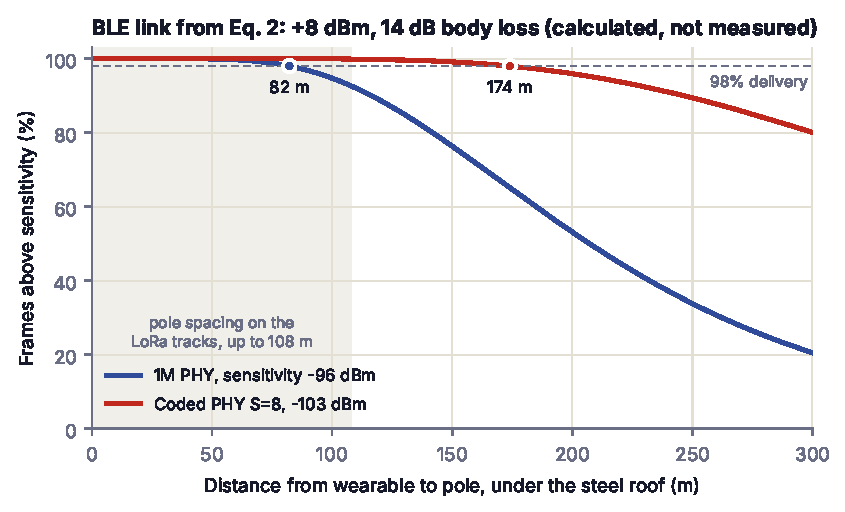
\includegraphics[width=0.72\linewidth]{link}
\caption{Share of frames above sensitivity against distance, from Eq.~\ref{eq:ble}.}\label{fig:link}\end{figure}

\section{Pseudonymous protocol}
\subsection{Threats}
Four adversaries are considered. $\mathcal A_1$ listens along the route and tries to follow one child or to link a
family. $\mathcal A_2$ records advertisements and plays them back elsewhere or later. $\mathcal A_3$ sends forged
commands to make a band buzz or to drain it. $\mathcal A_4$ steals a pole or a band and reads its memory.

\subsection{Keys}
The server keeps a 128-bit master key $\Kmaster$ in an encrypted keystore or a hardware security module. Each wearable
$u$ is given, at manufacture, its own key
\begin{equation}K_u=\cmac{\Kmaster}{\mathrm{UID}_u\,\|\,\mathrm{Salt}},\end{equation}
and its debug port is locked. Poles never hold $\Kmaster$ or any $K_u$. They authenticate to the network server with
their own LoRaWAN keys, protected by secure boot and flash encryption, and a tamper switch clears their memory.

\subsection{The 15-byte advertisement}
A wearable keeps a 16-bit counter $c$ driven by its 32.768~kHz crystal and increases it every 900~s. In each slot it
derives a fresh identifier and a fresh radio address:
\begin{align}\mathrm{ID}_{u,c}&=\operatorname{Trunc}_{32}\cmac{K_u}{\texttt{0x01}\,\|\,c},\\
M_{u,c}&=\operatorname{Trunc}_{46}\cmac{K_u}{\texttt{0x02}\,\|\,c}\ \text{with both top bits set.}\end{align}
It broadcasts the payload of Table~\ref{tab:frame} every 800~ms, and every 200~ms while SOS is pressed. Because the
counter is sent, nothing needs to be written to the wearable at registration. Three encodings left open in the first
draft are fixed by the reference code: truncation keeps the leading bytes of the CMAC, the counter enters each CMAC as
the same little-endian bytes it has on air, and the company identifier is sent low byte first.

\begin{table}[htb]\centering\footnotesize
\caption{The signed advertisement payload.}\label{tab:frame}
\begin{tabular}{@{}llp{0.62\linewidth}@{}}\toprule Bytes & Field & Content\\\midrule
0--1 & Company\_ID & \code{0xFF5A}, a laboratory value\\
2 & V\_type & bits 0--3 version (4); bit 4 role: band or parent tag\\
3--4 & Slot\_Counter & $c$, little-endian\\
5--8 & Rolling\_ID & $\mathrm{ID}_{u,c}$\\
9 & F\_stat & bit 0 SOS; 1 tether lost; 2 buzzer on; 3 low battery\\
10 & B\_mv & supply voltage in 20~mV steps\\
11--14 & MIC & $\operatorname{Trunc}_{32}\cmac{K_u}{\text{bytes }2\ldots10}$\\\bottomrule\end{tabular}\end{table}

\subsection{Resolving an identifier}
At the registration counter the operator scans the family's card and the codes on the band and the parent tag, and rests
both on a listener pad. Lifting a band off its storage magnet wakes it. The pad hears one frame, checks its MIC and that
the battery is above 2.90~V, and stores the counter it saw, $c_{init}$, with the time $t_{pair}$. At any later time $t$
the server expects
\begin{equation}\hat c_u(t)=\Bigl(c_{init}+\Bigl\lfloor\tfrac{t-t_{pair}}{900}\Bigr\rfloor\Bigr)\bmod 65536,\end{equation}
and keeps the identifiers of slots $\hat c_u-1$, $\hat c_u$, $\hat c_u+1$ in a hash map, which covers crystal drift of
$\pm20$~ppm. Among 10,000 wearables there is about a \Clash\% chance at any moment that two entries share a 32-bit
identifier, so the map holds a list per identifier and separates a clash by the counter.

\begin{algo}{Algorithm 1: verification and location at the server}
\textbf{Input:} pole, Rolling\_ID, $c$, RSSI, F\_stat, and for an SOS the whole frame.\par
1.\ Look up Rolling\_ID. If there is no entry whose slot equals $c$ within $\{\hat c_u-1,\hat c_u,\hat c_u+1\}$: count it
against the pole and \textbf{drop}.\par
2.\ If the SOS bit is set: recompute the MIC over bytes 2--10 with $K_u$. If it differs: count a forgery and
\textbf{drop}. Otherwise raise the \textbf{priority alarm}.\par
3.\ Among reports for $u$ in the last 15~s, place $u$ at the pole with the strongest signal.\par
4.\ If a wearable appears to have moved faster than any vehicle on the track, flag the sighting as suspect.
\end{algo}

\subsection{What the protocol gives, and what it does not}
\textbf{Unlinkability against $\mathcal A_1$.} AES-CMAC is a pseudorandom function \cite{rfc4493}, so without $K_u$ the
identifiers and addresses of different slots are indistinguishable from random strings. Within one 15-minute slot a
wearable can be followed.

\textbf{Unforgeable alarms against $\mathcal A_2$ and $\mathcal A_3$.} A forged SOS or a forged wake token passes with
probability $2^{-32}$ or $2^{-24}$ per attempt. A pole forwards at most ten SOS frames a minute and a wearable accepts
at most one command in 30~s.

\textbf{A stated limit: replay of ordinary sightings.} Arrival reports are 8 bytes and carry no MIC, and a pole has no
key with which to check one. A frame recorded at one pole and replayed at another inside its three-slot window, up to
45 minutes, is therefore accepted as a sighting. It cannot raise an alarm, and step~4 flags it when the implied speed
is impossible, but it can mislead. Carrying the MIC in arrival reports would close this at a cost of 4 bytes a wearable.

\section{Edge filtering and capacity}
\subsection{Time on air and collisions}
In the IN865 band \cite{rp002,wpc} the design uses $M=8$ channels of 125~kHz at coding rate 4/5 with an 8-symbol
preamble. A symbol lasts $T_{sym}=2^{SF}/BW$, 1.024~ms at SF7. For an application payload of $B$ bytes the LoRaWAN
frame is $13+B$ bytes and its time on air is \cite{semtech}
\begin{equation}T(B)=T_{sym}\Bigl(12.25+8+\max\Bigl(\Bigl\lceil\frac{8(13+B)-4\,SF+44}{4\,SF}\Bigr\rceil\cdot 5,\,0\Bigr)\Bigr).\end{equation}
At SF7 this gives \ToaSos~ms for an SOS (15 or 16 bytes), \ToaBloom~ms for a 64-byte heartbeat and \ToaChunk~ms for a
200-byte chunk of 25 arrivals. Uplinks are unsynchronised, so they collide as in pure ALOHA: with offered load $G$ per
channel a frame is lost with probability $1-e^{-2G}$. Capture and the partial orthogonality of spreading factors are
ignored, which makes the figures pessimistic.

\subsection{The pole's state machine}
A raw list of 4-byte identifiers every minute would exceed 222 bytes as soon as more than 55 people shelter at one pole.
Each pole therefore runs Algorithm~2 over a table of 1,024 entries.

\begin{algo}{Algorithm 2: edge filter at a pole}
\textbf{On each advertisement} with signal strength $r$:\par
1.\ Ignore it unless it is 15 bytes with Company\_ID \code{0xFF5A}.\par
2.\ If the SOS bit is set, fewer than 10 SOS were sent this minute, and this identifier was not forwarded in the last
90~s: \textbf{send now}, confirmed, on port 10, the frame and one byte of $r$; repeat at SF9 if unacknowledged.\par
3.\ If $r$ is below the gate ($-75$~dBm on tracks, $-65$~dBm in hubs): stop.\par
4.\ Update the entry: $\mathrm{RSSI}\leftarrow0.75\,\mathrm{RSSI}+0.25\,r$, count the hit, note the time.\par
5.\ When the hits reach $H$ ($H=1$ on tracks, $3$ in hubs) and the arrival is not yet reported: queue the 8-byte tuple
(identifier, $c$, RSSI, flags) and mark it reported.\par
\textbf{Every 15 s}, after a random 200--1500~ms:\par
6.\ Move entries unheard for 90~s to the departure queue.\par
7.\ Send arrivals in chunks of at most 25 tuples (200 bytes) on port 1.\par
8.\ Send departures, 4 bytes each, at most 50 a frame, on port 2.\par
\textbf{Every 60 s:}\par
9.\ Set three bits per reported identifier in a 512-bit filter, at $(\mathrm{CRC16}+j\cdot\mathrm{FNV1a})\bmod512$,
$j=0,1,2$, and send the 64 bytes on port 3.
\end{algo}

The gate of $-75$~dBm corresponds, by Eq.~\ref{eq:ble}, to about \GateTrackM~m, which is the ``core zone'' a pole
reports as its own. The appended signal-strength byte on port 10 is new in this revision: without it the server cannot
tell which of several poles that hear an SOS is nearest.

\subsection{Capacity of a gateway cell}
Consider $N$ wearables in a cell of $K=60$ poles, each reaching a new pole every $\tau=55$~s. A pole then sees Poisson
arrivals at $N/(\tau K)$ per second and holds $N/K$ wearables on average. Table~\ref{tab:cap} gives the offered load
and loss for four designs, with every stream of each design counted. A Monte Carlo simulation that puts every frame of
an hour on air, \McFrames{} frames in all, agrees with the loss formula to within \McErr{} percentage points.

\begin{table}[htb]\centering\footnotesize
\caption{Offered load $G$ and frame loss, in percent, as ``$G$ / loss'', for one 8-channel cell of 60 poles at SF7
against the number of wearables in the cell (calculated).}\label{tab:cap}
\TableCapacity\end{table}

\begin{figure}[htb]\centering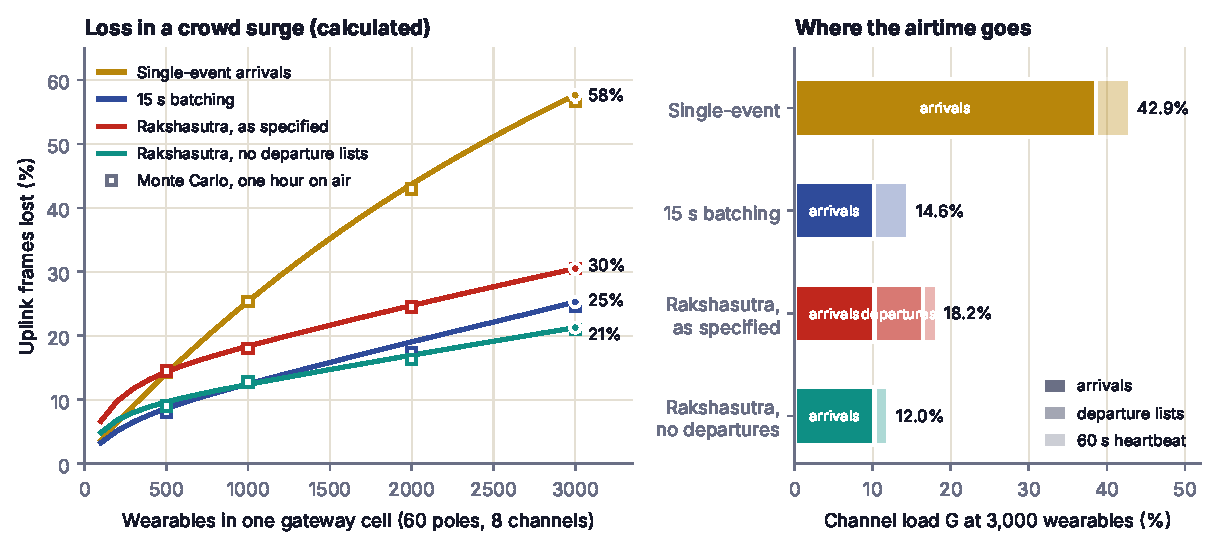
\includegraphics[width=\linewidth]{capacity}
\caption{Left: frame loss against the size of the surge; squares are the Monte Carlo check. Right: where the airtime
goes at 3,000 wearables.}\label{fig:cap}\end{figure}

Three things follow. First, batching does most of the work: from \LossSingle\% loss to \LossBatch\% at 3,000
wearables. Second, the Bloom heartbeat is what keeps every frame legal: at 3,000 wearables a raw list would be too long
for one frame at \OversizeBatch\% of poles, while the filter is always 64 bytes; it also needs less airtime than raw
lists once a cell holds more than about \BloomPays{} wearables. Third, the departure lists of step~8 cost more than the
heartbeat saves. As specified the design carries \AirVsBatch\% more airtime than plain batching and loses \LossRak\% of
frames. Without departure lists, inferring departure from the next arrival and the heartbeat, it carries
\AirVsBatchNd\% less and loses \LossRakNd\%. Against one uplink per arrival the airtime falls by \AirRed\% as specified
and by \AirRedNd\% without departure lists.

In the deployed layout a gateway serves about \DepPoles{} LoRa poles. With 5,000 wearables spread evenly over the route
a cell holds \DepTags{} of them and loses \DepLoss\% of frames, or \DepLossNd\% without departure lists.

A filter of 512 bits with three probes gives \BloomFifty\% false positives with 50 wearables at a pole,
\BloomHundred\% with 100 and \BloomThree\% with 300; it holds about \BloomCapFive{} at a 5\% error rate. The server
therefore uses a heartbeat only to confirm wearables it already places at that pole. The densest poles are on fibre and
can send a larger filter.

\section{Alerts and moving people}
\subsection{Why Class A is too slow}
A Class~A design needs 15~s to batch an arrival, 90~s to confirm a separation, up to 60~s for a downlink window and 8~s
to connect to the band: 173~s in the worst case. At 1.25~m/s a parent walks \ClassAWalk~m in that time, past several
poles. Rakshasutra uses two layers instead.

\subsection{Layer 1: a direct tether}
At pairing the pad writes the band's next 96 identifiers, 384 bytes covering 24 hours, into the parent tag. The tag
scans periodically, and if it misses the band four times in a row it sounds its own buzzer, with no network involved.

\begin{finding}
\textbf{Two corrections to the first draft.} It specified a 5~ms scan every 5~s. The band advertises every 800~ms, so a
5~ms window contains a whole advertisement only \TetherHit\% of the time, and four scans in a row all miss
\TetherAlarm\% of the time with the child beside the parent (simulated: in false alarm \TetherAlarmSim\% of the time).
A window of \TetherWindow~ms cannot miss, but costs \TetherUa~\textmu A and would empty the parent tag in about
\ParentLife{} months; synchronised scanning is the better route and is future work. Second, the signal is lost at the
edge of radio range, about \TetherRange~m by Eq.~\ref{eq:ble}, not at 25--30~m. To alert at 30~m the tag must treat a
signal weaker than about $-$\TetherGate~dBm as a miss.
\end{finding}

\subsection{Layer 2: Class C multicast}
When the server finds $d_G\geq200$~m between a band and its parent tag, or a guard starts a search, it sends an 8-byte
wake token to the poles within two hops of the wearable, all of which listen continuously in Class~C. They broadcast
it as a connectionless advertisement and the wearable, which opens a short scan window every 4~s, sounds its buzzer.
The token is the identifier, a command byte and 24 bits of AES-CMAC. The design target is 2.5 to 5~s from decision to
buzzer; it has not been simulated or measured, and the wearable's short scan window raises the same timing question as
the tether.

\subsection{Passengers at 20 km/h}
An electric vehicle at 5.56~m/s crosses a pole's 25~m core zone in 4.5~s. A band that slows its advertising to one
every 2 to 5~s when its accelerometer sees no motion sends at most two or three frames in that time, so a three-hit
rule reports it on at most \SlowTwo\% of passes. With a fixed 800~ms interval the pass holds five or six frames, and
with $H=1$ one decoded frame is enough. If a frame is lost only when another wearable in range is on air at the same
moment, the capture rate is \EvCap\% with 150 other wearables in range of the pole and \EvCapDense\% with 300
(calculated; Fig.~\ref{fig:tether}).

\begin{figure}[htb]\centering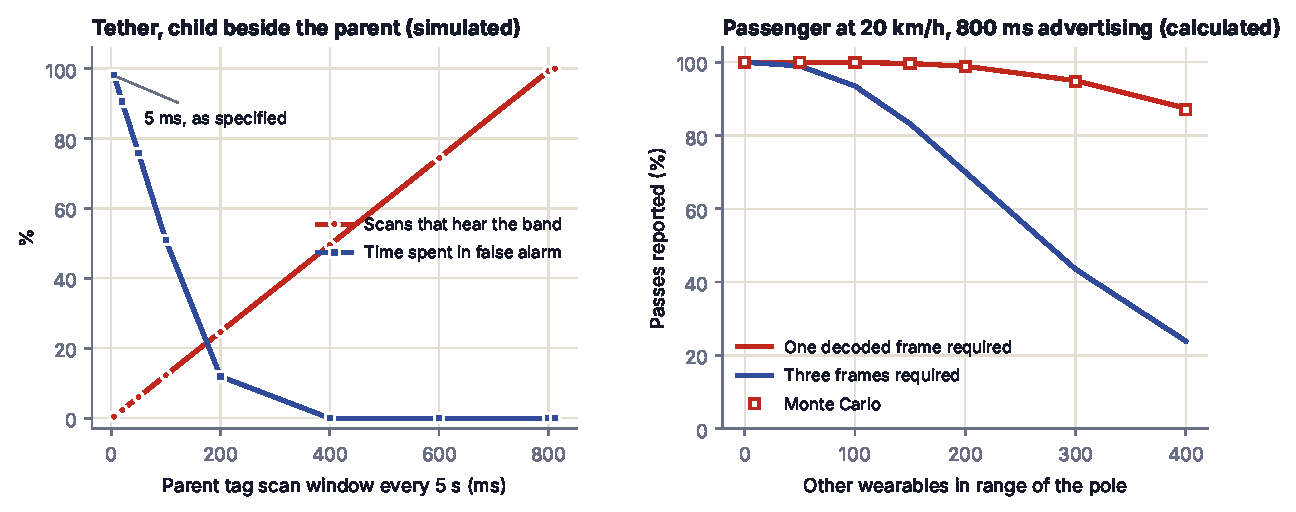
\includegraphics[width=\linewidth]{tether_ev}
\caption{Left: the tether scan window against how often the parent tag hears the band and how long it spends in false
alarm (simulated). Right: capture of a passenger at 20~km/h against the crowd around the pole.}\label{fig:tether}\end{figure}

\subsection{An SOS, end to end}
Pressing the button sets the SOS bit and the 200~ms interval. A pole forwards the frame at once. Under a 3,000-wearable
surge the first LoRa attempt is lost \SosFirstLoss\% of the time; a repeat follows at SF9 after an assumed 3~s. In
simulation the alarm reaches the control room in a median of \SosMedian~s, within 4~s in \SosFour\% of cases, and
within \SosPninefive~s in 95\%. On fibre poles, where the densest crowds are, 95\% arrive within \SosFiberP~s.

\subsection{Backend}
Gateways and fibre poles publish to an MQTT broker; identity resolution and the graph distance run in memory; a worker
writes batches of 500 to 2,500 records to a time-series database every 5~s. These components are specified, not built.

\section{Power}
\begin{table}[htb]\centering\footnotesize
\caption{Wearable current on a 620~mAh CR2450, as tabled in the first draft (design values).}\label{tab:power}
\TablePower\end{table}
Table~\ref{tab:power} sums to \Iactive~\textmu A. At 14 hours a day on the trek and 10 on the storage rack this gives
\LifeWarm{} months at 25~\textdegree C, and \LifeCold{} months at $-5$~\textdegree C where the cell loses 30\% of its
capacity. But 1.25~ms per advertisement is the length of a 1M PHY event on three channels. On Coded PHY, which the
range in Section~3 assumes, the same 15 bytes take \AdvCoded~ms: three \code{ADV\_EXT\_IND} packets and one
\code{AUX\_ADV\_IND}. The mean current is then \IactiveCoded~\textmu A and the life \LifeWarmCoded{} months warm and
\LifeColdCoded{} months cold (Fig.~\ref{fig:power}).

\begin{figure}[htb]\centering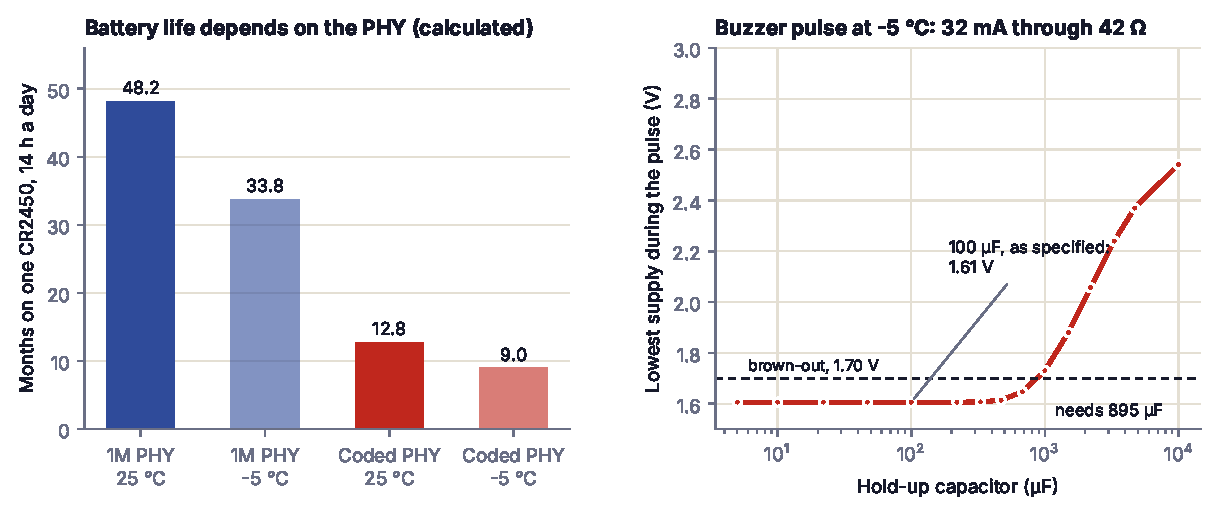
\includegraphics[width=\linewidth]{power}
\caption{Left: battery life by PHY and temperature. Right: lowest supply voltage during a buzzer pulse in the cold
against the size of the hold-up capacitor (calculated).}\label{fig:power}\end{figure}

\textbf{The cold buzzer pulse.} At $-5$~\textdegree C the cell's internal resistance rises to about 42~$\Omega$. A
32~mA buzzer and LED pulse then drops $0.032\times42=1.34$~V, taking a 2.95~V cell to \DroopUnbuf~V, below the
1.70~V minimum of the radio chip. The first draft added a 100~\textmu F capacitor and a 20\% duty cycle and reasoned
from the average current. That does not hold: 100~\textmu F behind 42~$\Omega$ has a time constant of \TauMs~ms, far
shorter than a 100~ms pulse, so the supply still falls to \DroopCap~V. Either the capacitor must be at least
\CapNeed~\textmu F, or the pulse current must stay below \PulseMax~mA.

\textbf{Choice of chip.} The first draft named the nRF52811 with $+8$~dBm output. That part is specified to $+4$~dBm;
$+8$~dBm needs a part such as the nRF52820 or nRF52833. This is to be confirmed against the datasheets before the
bill of materials is fixed, and the currents in Table~\ref{tab:power} re-derived for the chosen part.

\section{Law, ethics and physical safety}
\textbf{Data protection.} Section~9 of India's Digital Personal Data Protection Act, 2023 \cite{dpdp} requires
verifiable consent from a parent or guardian before a child's data are processed, and forbids tracking for behavioural
monitoring or advertising. Rakshasutra records consent at registration, keeps only a first name, a band identifier, a
guardian's phone number and the card number, sends no personal data over the air, and deletes location trails within
24 to 72 hours of the band's return.

\textbf{Kiosks.} Lookup kiosks in the phone-free zones respond only to the family's own card or parent tag, show only
the members bound to it, do not search by name, lock after three failed scans, log every query and blank after 30~s.

\textbf{Button cells.} A swallowed coin cell can cause severe internal burns \cite{iec}. The band is welded shut or
closed with captive tool-only screws, has no battery door, and uses a non-porous strap that is disinfected between
uses.

\section{What changed since the first draft}\label{sec:audit}
The first draft of this paper (October 2026) called the system SurakshaNet in its text and described its results as
empirical. Neither was right: the name is Rakshasutra, and nothing has been measured. For this revision every
checkable number was recomputed by the open code. Of \AuditTotal{} claims, \AuditRep{} were reproduced, \AuditDiff{}
differ and now carry the model's value, \AuditFix{} need a design fix, and \AuditOpen{} cannot be settled without a
datasheet or a measurement. The full list is in \code{AUDIT.md} in the repository. The main changes:
\begin{itemize}
\item Loss in a 3,000-wearable surge is \LossRakNd--\LossRak\%, not 15.8\%; the first draft counted only part of the
traffic of Algorithm~2. Departure lists should be dropped.
\item The airtime saving over single-event forwarding is \AirRed--\AirRedNd\%, not 82.4\%.
\item The tether cannot work with a 5~ms scan window, and alerts at the edge of radio range unless it uses a
signal-strength gate.
\item A 100~\textmu F capacitor does not prevent brown-out during the cold buzzer pulse.
\item Battery life on Coded PHY is \LifeColdCoded--\LifeWarmCoded{} months, not ``over 11 months'' in the cold.
\item Bluetooth ranges from Eq.~\ref{eq:ble} are longer than first tabled; the 50~m margin is \MarginFifty~dB, not
28.6~dB.
\item Ordinary sightings can be replayed inside their slot window; only alarms are fully authenticated.
\item An SOS arrives within 4~s in \SosFour\% of simulated cases under a surge, not in all.
\end{itemize}

\section{Conclusion}
Rakshasutra combines a signed, rotating Bluetooth advertisement with poles that filter at the edge and forward over
LoRaWAN, to follow vulnerable pilgrims between the gates of a covered mountain route without phones or cellular
coverage. The calculations support the core of the design: frames stay within the payload limit at any density,
batching and a Bloom heartbeat cut airtime by well over half, passengers in vehicles are captured, and forged alarms
are rejected. They also show where it must change before hardware is built: the tether's scanning, the departure
lists, the buzzer's power supply and the choice of radio chip. The next step is measurement: roof loss and range under
a real shelter, then a pilot on one zone. Later work may extend the approach to tunnel construction sites and to
temporary gatherings such as the Kumbh Mela.

\begin{thebibliography}{99}\footnotesize
\bibitem{rp002} LoRa Alliance, \emph{RP002-1.0.4 LoRaWAN Regional Parameters}, 2022.
\bibitem{semtech} Semtech, \emph{LoRa Modem Designer's Guide}, AN1200.13.
\bibitem{rfc4493} J.~Song, R.~Poovendran, J.~Lee, T.~Iwata, ``The AES-CMAC algorithm,'' RFC~4493, IETF, 2006.
\bibitem{btcore} Bluetooth SIG, \emph{Bluetooth Core Specification}, version 5.1, 2019.
\bibitem{bloom} B.~H.~Bloom, ``Space/time trade-offs in hash coding with allowable errors,'' \emph{Commun.\ ACM}
13(7):422--426, 1970.
\bibitem{kirsch} A.~Kirsch, M.~Mitzenmacher, ``Less hashing, same performance: building a better Bloom filter,''
\emph{Random Struct.\ Algorithms} 33(2):187--218, 2008.
\bibitem{dpdp} Government of India, \emph{The Digital Personal Data Protection Act, 2023} (No.~22 of 2023), Section~9.
\bibitem{wpc} Wireless Planning and Coordination Wing, Government of India, rules for low-power equipment in the
865--867~MHz band.
\bibitem{augustin} A.~Augustin, J.~Yi, T.~Clausen, W.~M.~Townsley, ``A study of LoRa: long range and low power networks
for the Internet of Things,'' \emph{Sensors} 16(9):1466, 2016.
\bibitem{centenaro} M.~Centenaro, L.~Vangelista, A.~Zanella, M.~Zorzi, ``Long-range communications in unlicensed bands,''
\emph{IEEE Wireless Commun.}\ 23(5):60--67, 2016.
\bibitem{adelantado} F.~Adelantado et al., ``Understanding the limits of LoRaWAN,'' \emph{IEEE Commun.\ Mag.}\
55(9):34--40, 2017.
\bibitem{heinrich} A.~Heinrich, M.~Stute, T.~Kornhuber, M.~Hollick, ``Who can find my devices? Security and privacy of
Apple's crowd-sourced Bluetooth location tracking system,'' \emph{Proc.\ Privacy Enhancing Technol.}\ 2021(3):227--245.
\bibitem{nordic} Nordic Semiconductor, \emph{nRF52811 Product Specification}.
\bibitem{iec} IEC 60086-4, \emph{Primary batteries, Part 4: Safety of lithium batteries}.
\end{thebibliography}
\nocite{centenaro,nordic}
\end{document}
